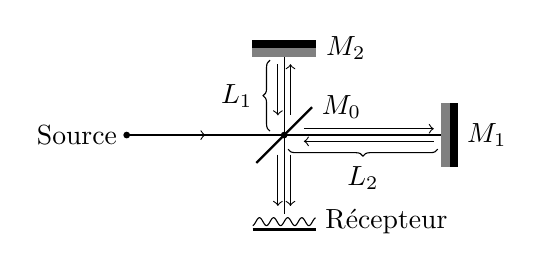
\begin{tikzpicture}
	\usetikzlibrary{decorations}
	\usetikzlibrary{decorations.pathmorphing}
	\usetikzlibrary{decorations.pathreplacing}
	\usetikzlibrary{decorations.shapes}
	\usetikzlibrary{decorations.text}
	\usetikzlibrary{decorations.markings}
	\usetikzlibrary{decorations.fractals}
	\usetikzlibrary{decorations.footprints}
	 
	%%% Général %%%
	\draw (0,0) -- (4,0); % Trajet horizontal
	\filldraw[black] (0,0) circle (1pt) node[anchor=east] {Source}; % Point S
	\draw (2,-1) -- (2,1); % Trajet vertical
	\filldraw[black] (2,0) circle (1pt); % Point central
	 
	%%% Flèches %%%
	\draw[->] (0,0) -- (1,0); % Fleche qui part de S
	\draw[->] (2.25,0.08) -- (3.9,0.08); % M1 aller
	\draw[<-] (2.25,-0.08) -- (3.9,-0.08); % M1 retour
	\draw[<-] (2.08,0.9) -- (2.08,0.25); % M2 aller
	\draw[->] (1.92,0.9) -- (1.92,0.25); % M2 retour
	\draw[->] (1.92,-0.25) -- (1.92,-0.9); % R
	\draw[->] (2.08,-0.25) -- (2.08,-0.9); % R
	 
	%%% Accolades %%%
	\draw[decorate,decoration={brace,mirror,raise=0.1cm,}] (2.05,-0.08) -- (3.95,-0.08) node[below=0.2cm,pos=0.5] {$L_2$};
	\draw[decorate,decoration={brace,raise=0.1cm,}] (1.92,0.05) -- (1.92,0.95) node[left=0.2cm,pos=0.5] {$L_1$};
	 
	%%% Beamsplitter %%%%
	\draw[thick] (1.6464,-0.3535) -- (2.3535,0.3535);
	\draw (2.3535,0.3535) node[anchor=west] {$M_0$};
	 
	%%% M1 %%%
	\filldraw[black] (4.1,-0.4) rectangle (4.2,0.4);
	\filldraw[gray] (4,-0.4) rectangle (4.1,0.4);
	\draw (4.2,0) node[anchor=west] {$M_1$};
	 
	%%% M2 %%%
	\filldraw[black] (1.6,1.1) rectangle (2.4,1.2);
	\filldraw[gray] (1.6,1) rectangle (2.4,1.1);
	\draw (2.41,1.1) node[anchor=west] {$M_2$};
	 
	%%% R %%%
	\draw [domain=-0.4:0.4][samples=200] plot (\x+2,{sin(\x*35 r)*0.05-1.1});
	\draw[thick] (1.6,-1.2) -- (2.4,-1.2);
	\draw (2.4,-1.1) node[anchor=west] {Récepteur};
\end{tikzpicture}